\documentclass{article}
\usepackage[utf8]{inputenc}
\usepackage{graphicx}
\usepackage{float}
\usepackage{mathptmx}
\usepackage{amsmath}

\title{Computer Graphics: A Review}

\author{Yanjie Ze }
\date{\today}

\begin{document}

\maketitle
This is the course note for CS337: Computer Graphics, taught by Prof. Bin Sheng, written by Yanjie Ze. 

\section{Introduction}
\begin{itemize}
    \item What is Computer Graphics?
    
    Generating images with the aid of computers.
    
    \item Grading Policy.
    
    \begin{itemize}
        \item Quiz 30\%
        \item Exam 30\%
        \item Project 40\%
    \end{itemize}
\end{itemize}


\section{Graphics Pipeline}
\begin{itemize}
\item Hardware:
\begin{figure}[H]
    \centering
    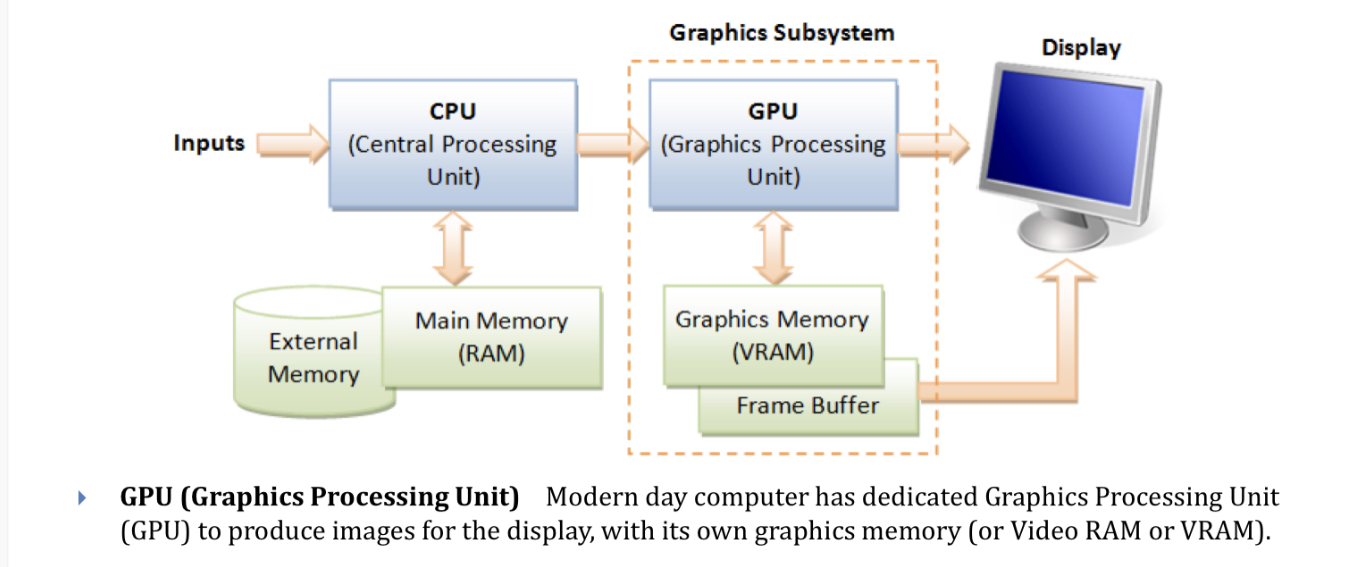
\includegraphics[width=0.8\textwidth]{imgs/hardware.jpeg}
\end{figure}

    \item Pipeline:

\begin{itemize}
    \item Input of Pipeline:
\begin{itemize}
    \item Primitives: 
    
    The inputs to the Graphics Rendering Pipeline are geometric primitives (such as triangle, point, line or quad), which is formed by one or more vertices.

Each vertex is associated with its attributes such as the position, color, normal and texture.
    \item Vertices:  
    
    \begin{itemize}
        \item 

    Position in 3D space V=(x, y, z): typically expressed in floating point numbers.

\item
Color: expressed in RGB (Red-Green-Blue) or RGBA (Red-Green-Blue-Alpha) components. 

\item 
Vertex-Normal N=(nx, ny, nz): Normals are used to differentiate the front- and back-face, and for other processing such as lighting.
\item 
Texture T=(s, t): In computer graphics, we often wrap a 2D image to an object to make it seen realistic. A vertex could have a 2D texture coordinates (s, t), which provides a reference point to a 2D texture image.

    \end{itemize}
\end{itemize}

\item Pixel vs. Fragment:

Pixels refers to the dots on the display. A pixel is 2-dimensional, with a (x, y) position and a RGB color value .

A fragment is 3-dimensional, with a (x, y, z) position. The (x, y) are aligned with the 2D pixel-grid. The z-value (not grid-aligned) denotes its depth.


Fragments are produced via interpolation of the vertices. Hence, a fragment has all the vertex's attributes such as color, fragment-normal and texture coordinates.


\item Pipeline:
\begin{itemize}
    \item Vertex Processor
    \item Rasterizer
    \item Fragment Processor
    \item Output Merging
\end{itemize}
\begin{figure}[H]
    \centering
    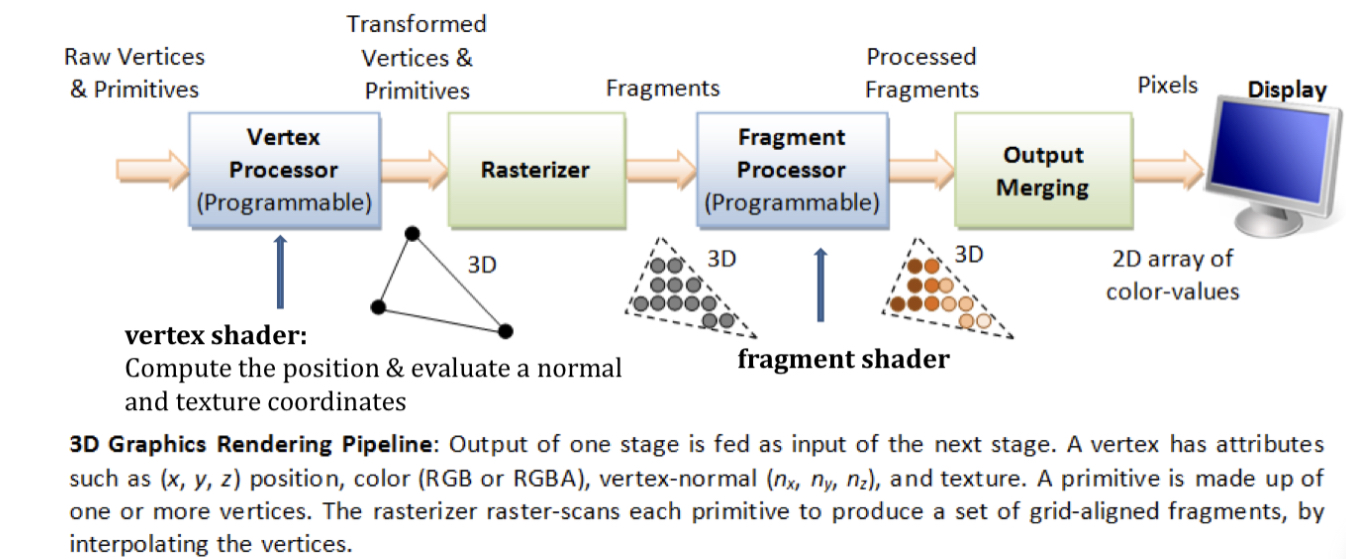
\includegraphics[width=0.8\textwidth]{imgs/pipeline.jpeg}
    
    
\end{figure}

\item Vertex Process:
\begin{itemize}
    \item Model Transform
    \item View Transform
    \item Projection Transform
    \item Viewport Transform
\end{itemize}

\item Coordinate System: Right hand coordinate system
\end{itemize}
\item 
Visibility
\begin{itemize}
    \item Painter's Algorithm: paint from back to front, overwrite in the framebuffer
    \item Z-Buffer: 
    \begin{itemize}
        \item Store current min z-value for each sample position with a \textbf{depth buffer (z-buffer)}
        \item Fastest way: \textbf{draw from front to back}
\item Algorithm:
\begin{figure}[H]
    \centering
    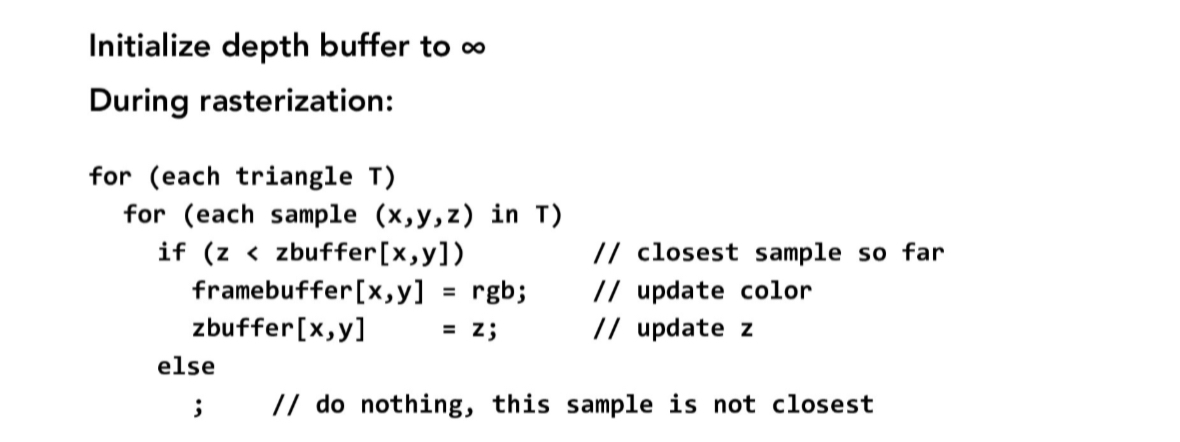
\includegraphics[width=0.9\textwidth]{imgs/z-buffer.jpg}
    \caption{Z-buffer}

\end{figure}
        
    \end{itemize}
    
\end{itemize}
\end{itemize}
\section{Basic Transformation}

\begin{itemize}
\item Cross Product:
\begin{figure}[H]
        \centering
        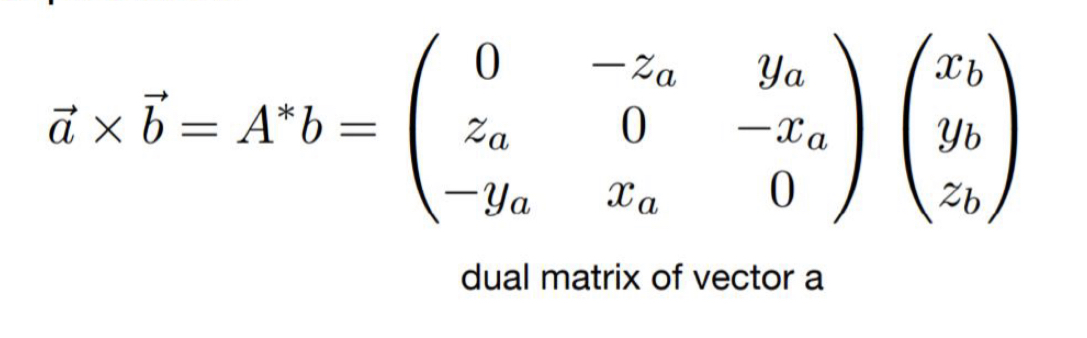
\includegraphics[width=0.5\textwidth]{imgs/cross_product.jpeg}
        
    \end{figure}
    \item 
2D Transform:
\begin{itemize}
    \item scale: uniform, non-uniform.$\begin{bmatrix} s_x & 0 \\ 0 & s_y\end{bmatrix}$
    \item reflection:$\begin{bmatrix} -1 & 0 \\ 0 & 1\end{bmatrix}$
    \item rotate: $\begin{bmatrix} \cos \theta & -\sin\theta \\ \sin\theta & \cos \theta\end{bmatrix}$
    \item shear: $\begin{bmatrix} 1 & a \\ 0 & 1\end{bmatrix}$
    \item linear:$\begin{bmatrix} a & b \\ c & d\end{bmatrix}$
    \item affine:$\begin{bmatrix} a & b &t_x\\ c & d &t_y \\ 0&0&1\end{bmatrix}$
    
\end{itemize}

\item Homogeneous Coordinates

\item Compose Transform

\item 3D Rotations: 
\begin{itemize}
    \item Euler angles:roll, pitch, yaw
    \begin{figure}[H]
        \centering
        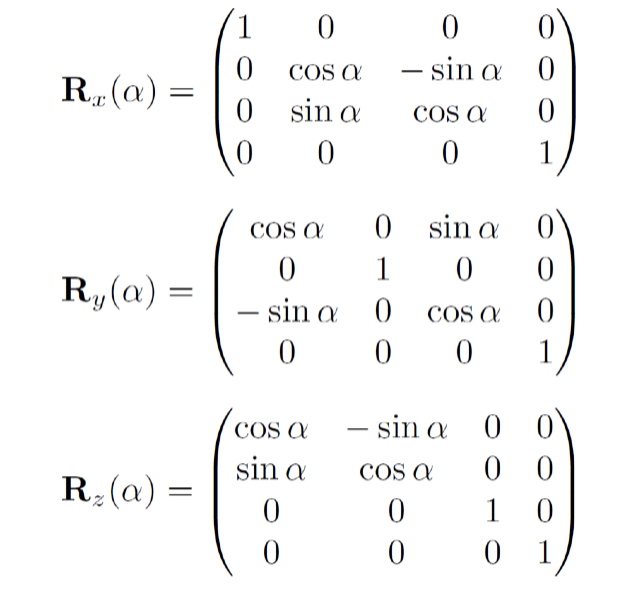
\includegraphics[width=0.5\textwidth]{imgs/3D_rotation.jpeg}
        
    \end{figure}
    \item Rodrigues' Rotation Formula:
    \begin{figure}[H]
        \centering
        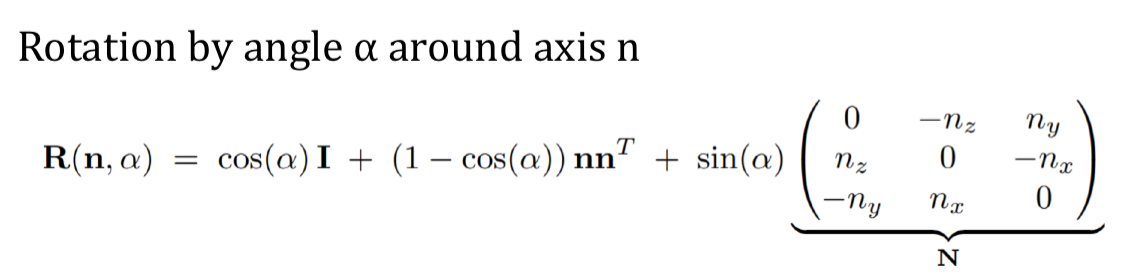
\includegraphics[width=0.6 \textwidth]{imgs/rog_rotation.jpeg}
        
    \end{figure}
\end{itemize}
\end{itemize}

\section{Viewing and Perspective}
\begin{itemize}
    \item MVP transformation:
\begin{itemize}
    \item model transformation: find a good place and arrange people
    \item view transformation: find a good angle to put the camera
    \item projection transformation: Cheese!
\end{itemize}
\item 
\textbf{View transformation}:
\begin{itemize}
\item $t$, up vector. $g$, view vector. $e$, eye point.
\item Translation Vector: $T_{view}=[-x_e,-y_e,-z_e,1]^T$
\item Rotation Matrix: First, rotate from the origin point to the camera position and get the matrix. Second, rotate back and get the inverse matrix.
\begin{figure}[H]
    \centering
    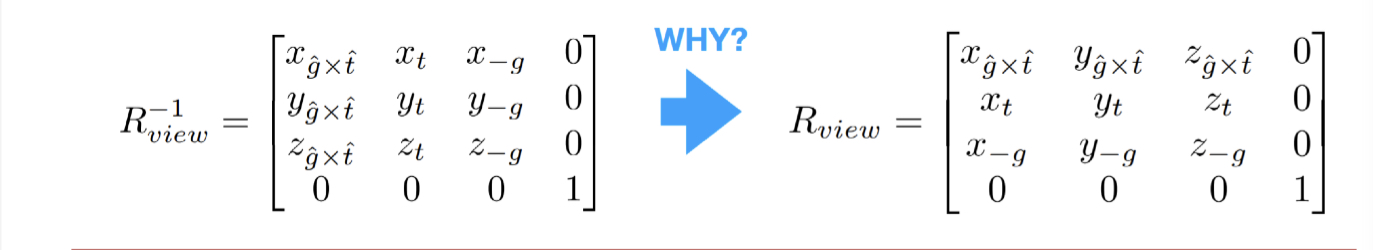
\includegraphics[width=0.9\textwidth]{imgs/view_trans.jpeg}
    \caption{View Transformation}

\end{figure}
\end{itemize}

\item Orthographic projection:
\begin{itemize}
    \item Map a cuboid into the canonical cube.
    \item Translation then Scale:
    \begin{figure}[H]
    \centering
    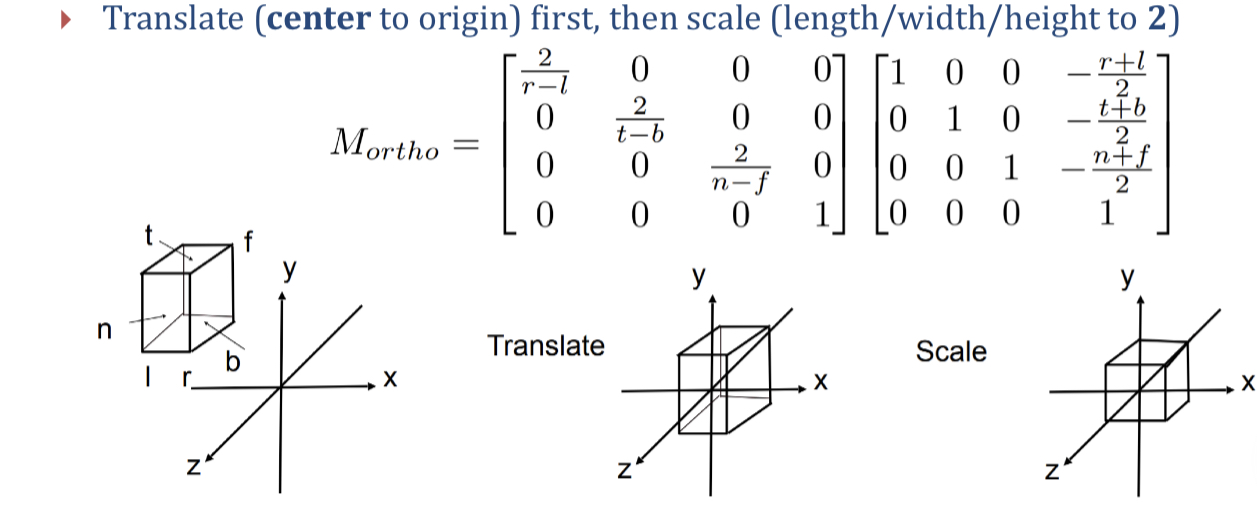
\includegraphics[width=0.9\textwidth]{imgs/ortho_proj.jpeg}
    \caption{Orthographic projection}

\end{figure}

\end{itemize}
\item Perspective Projection:
\begin{itemize}
    \item First, squish the frustum into a cuboid with $n\rightarrow n, f\rightarrow f$. Second, do orthographic projection.
    \item Induction:
\begin{figure}[H]
\centering
\begin{minipage}[t]{0.48\textwidth}
\centering
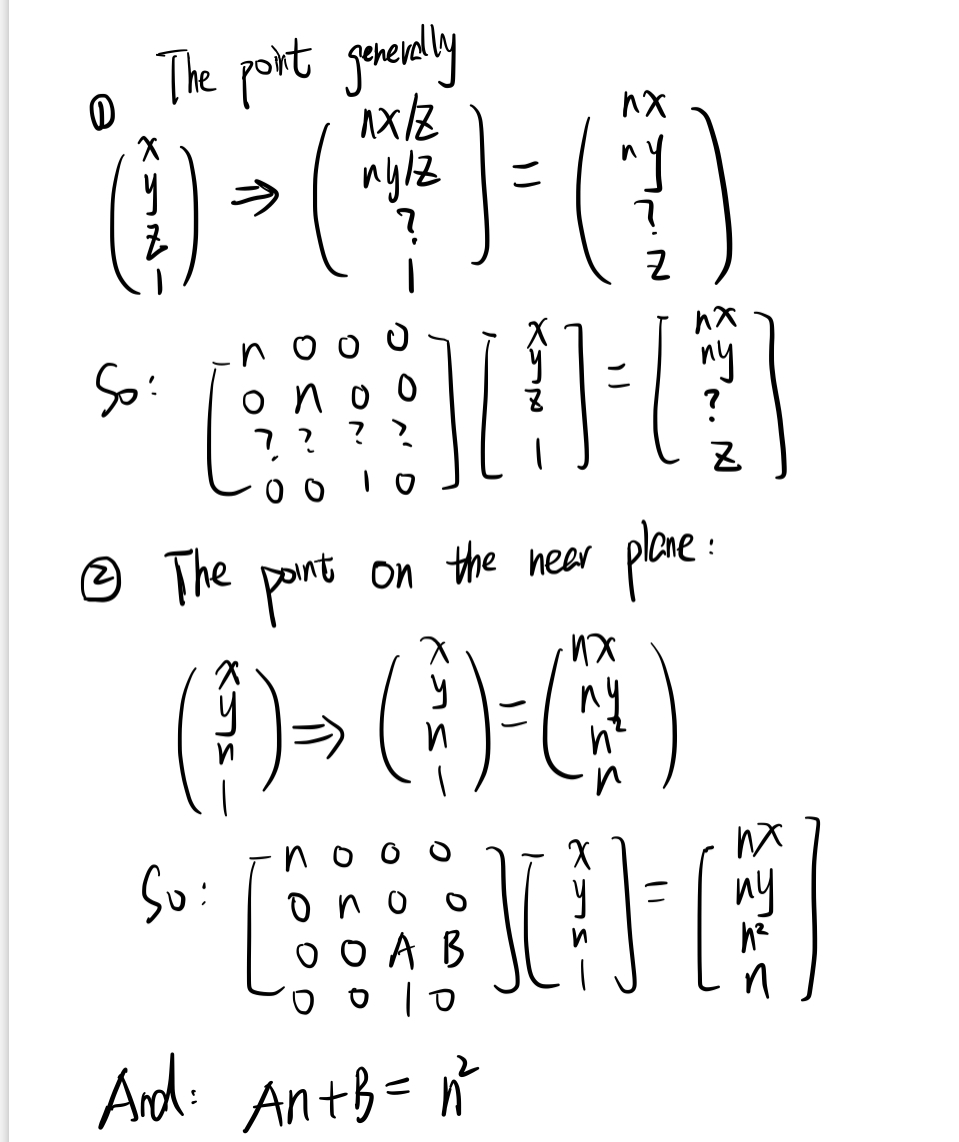
\includegraphics[width=6cm]{imgs/process1.jpeg}
\caption{Induction 1}
\end{minipage}
\begin{minipage}[t]{0.48\textwidth}
\centering
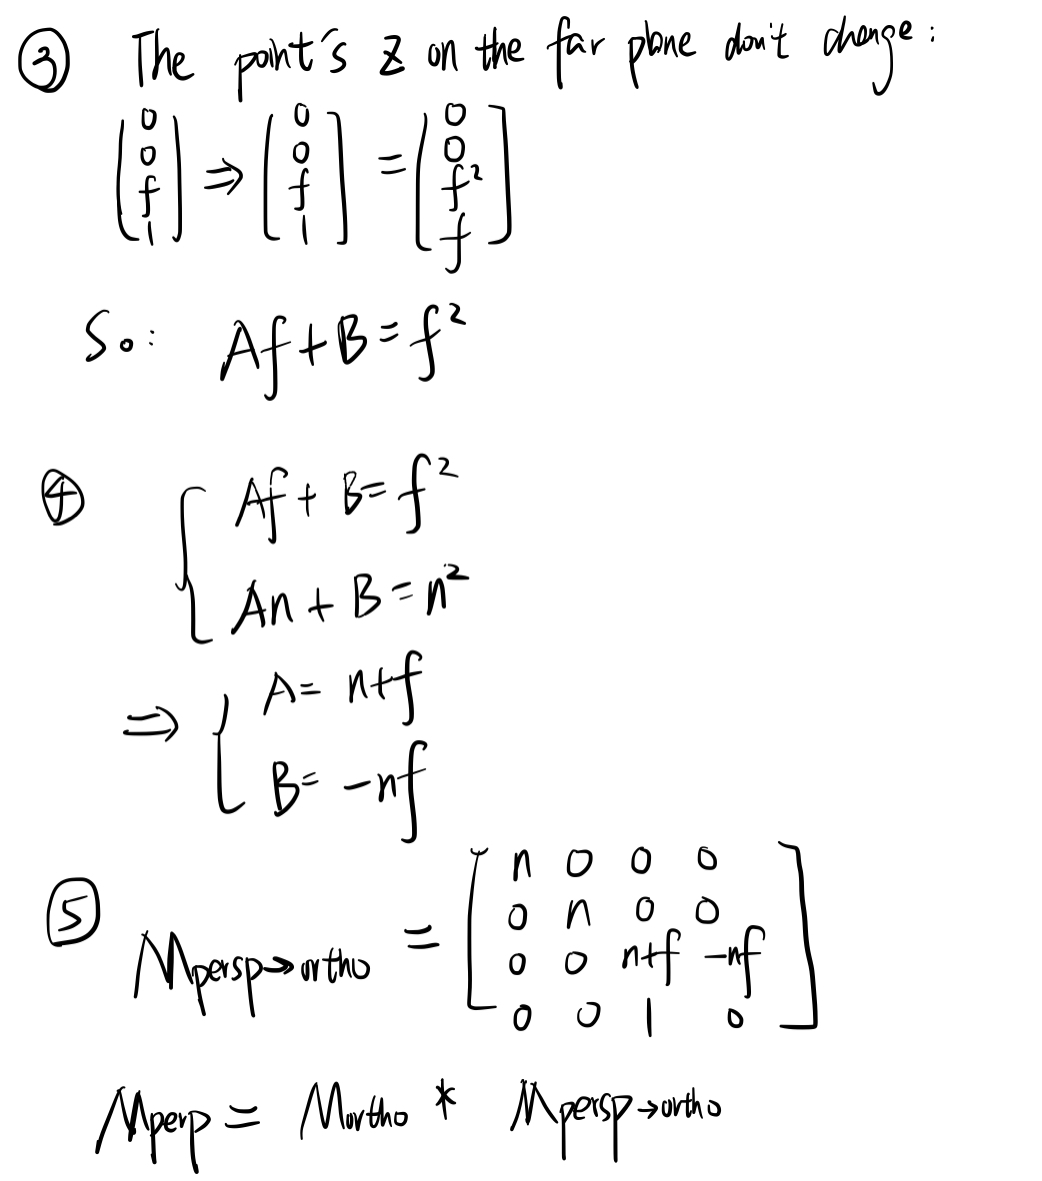
\includegraphics[width=6cm]{imgs/process2.jpeg}
\caption{Induction 2}
\end{minipage}
\end{figure}

\item The result:
\begin{figure}[H]
    \centering
    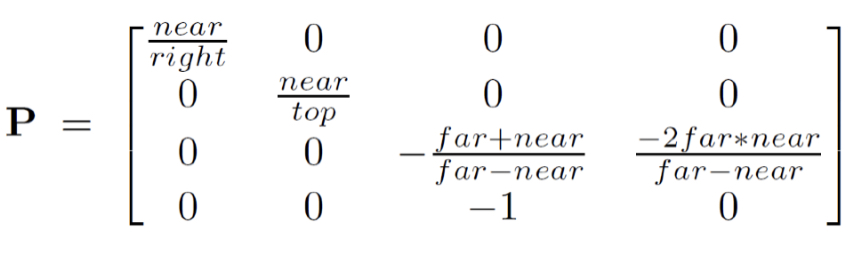
\includegraphics[width=0.6\textwidth]{imgs/pers_proj.jpeg}
    % \caption{Perspective Projection}

\end{figure}
\end{itemize}

\item Canonical Cube to Screen
\begin{itemize}
    \item Irrelevant to $z$
    \item From $[-1,1]^2$ to $[0,width]\times[0,height]^2$:
    \begin{figure}[H]
    \centering
    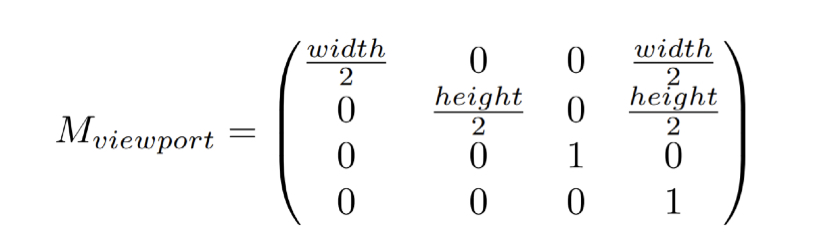
\includegraphics[width=0.6\textwidth]{imgs/viewport.jpeg}
    % \caption{Viewport Transformation}
\end{figure}
\end{itemize}

\end{itemize}


\section{Shading Basics}
\section{Shading Basics}

\begin{itemize}
    \item Shading Model:
    
Gooch Shading Model:
\begin{figure}[H]
        \centering
        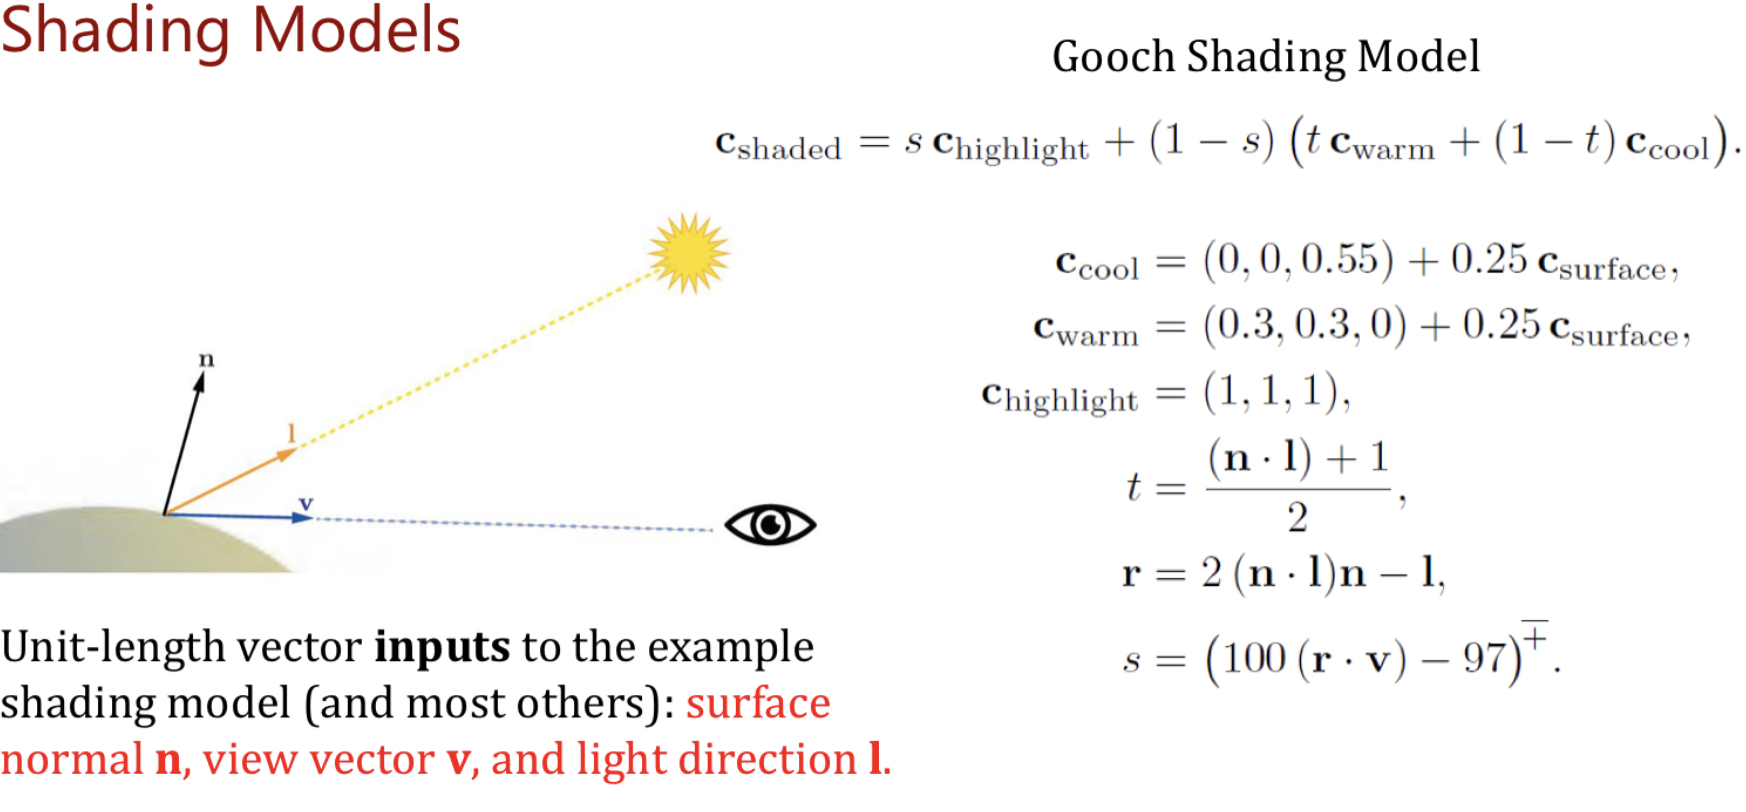
\includegraphics[width=0.9\textwidth]{imgs/gooch_shading.jpeg}
        
    \end{figure}

\item Light Sources:
\begin{itemize}
    \item Directional Lights: no location, constant
    
    \item Punctual Lights: have a location
    \begin{itemize}
        \item Point Light: $c_{light}$ varies with the distance.
        \item Spotlight: project light in a circular cone.
    \end{itemize}
\end{itemize}

\item Aliasing and Anti-aliasing:
\begin{itemize}
    \item Evaluate the point inside the triangle: by cross product.
    \item Incremental Triangle Traversal (faster)
\end{itemize}

\item \textbf{Blurring before sampling} for antialiasing

But why can this work?

\begin{itemize}
    \item Undersampling creates frequency aliases.
    \item Filtering = get rid of certain frequency contents
    \item Sampling = repeating frequency contents
    \item Aliasing = mixed frequency contents
    \item Anti-aliasing = limiting, then repeating
    
\end{itemize}

\item Anti-aliasing by \textbf{supersampling} (MSAA)
\begin{itemize}
    \item Sample multiple locations in one pixel, then average them.
    \item Cons: \textbf{cost too much! no free lunch}
\end{itemize}

\item Transparency: The meaning of alpha $\alpha$:
\begin{figure}
    \centering
    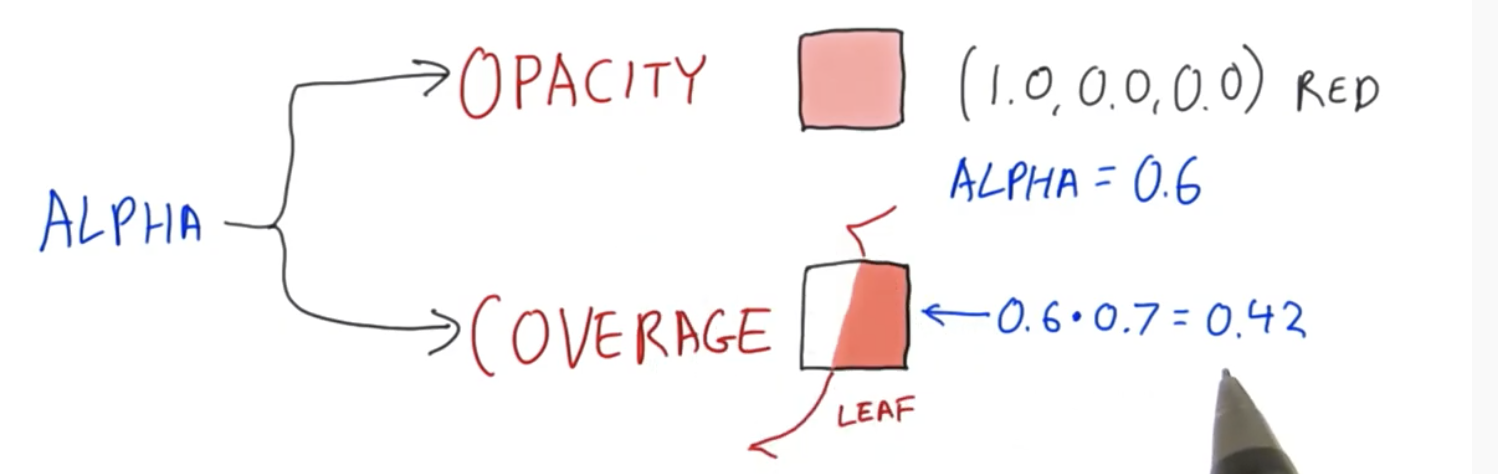
\includegraphics[width=0.8\textwidth]{imgs/alpha.png}
\end{figure}



\end{itemize}

\section{Illumination \& Shading}
\begin{itemize}
    \item Blinn-Phong reflectance model:
    \begin{itemize}
        \item A local illumination model: just one bounce, light $\rightarrow$ surface $\rightarrow$ viewer.
         \item \textbf{Shading normal is on each vertex. }Geometric normal is on the surface.
        \item Consisit of three kinds of light:
        
        \begin{itemize}
            \item Specular highlight
            \item Diffuse reflection
            \item Ambient lighting
        \end{itemize}
       
        
        \item Diffuse reflection:
        \begin{itemize}
            \item Lambert's cosine law: light per unit area is proportional to $\cos \theta = \mathbf{I} \cdot \mathbf{n}$.
            \item Shading \textbf{independent} of view direction.
            \item Lambertian shading: $$L_d=k_d(I/r^2)\max(0,\mathbf{I} \cdot \mathbf{n})\,,$$where $k_d$ is the diffuse coefficient.
        \end{itemize}
        
        \item Specular shading:
        \begin{itemize}
            \item Intensity \textbf{depends} on view direction: brighter when near mirror reflection direction.
            \item Half angle vector or bisector:
            $$
            \mathbf{h}=\frac{\mathbf{v}+\mathbf{l}}{\|\mathbf{v}+\mathbf{l}\|}
            $$
            \item Formula:
            $$
            L_d=k_d(I/r^2)\max(0,\mathbf{n} \cdot \mathbf{h})^p\,.
            $$
            $p$ larger, light more focuses.
        \end{itemize}
        
    \item Ambient shading:
    \begin{itemize}
        \item Shading that does \textbf{not depend} on anything. 
        \item This is actually a fake light, just to make the effect better.
        \item Formula:
        $$
        L_a = k_a I_a\,.
        $$
    \end{itemize}
    
    \item Blinn-Phong reflection model:
    $$
    L = L_a + L_d + L_s
    $$
    \end{itemize}
    \newpage
    \item Shading frequencies:
    
    \begin{itemize}
        \item Flat shading: each triangle has just one normal vector. Not good for smooth surfaces.
        \item Gouraud shading (shade earch vertex): each vertex has one normal vector, then we interpolate colors from vertices across triangle.
        
        Vertex normal: average over surrounding face normals. 
        \item Phong shading (shade each pixel): 
        \begin{itemize}
            \item each pixel's normal vector is interpolated using vertex normal
            \item compute full shading model at each pixel
            \item The interpolation result should be \textbf{normalized} before used.
            \begin{figure}[H]
                \centering
                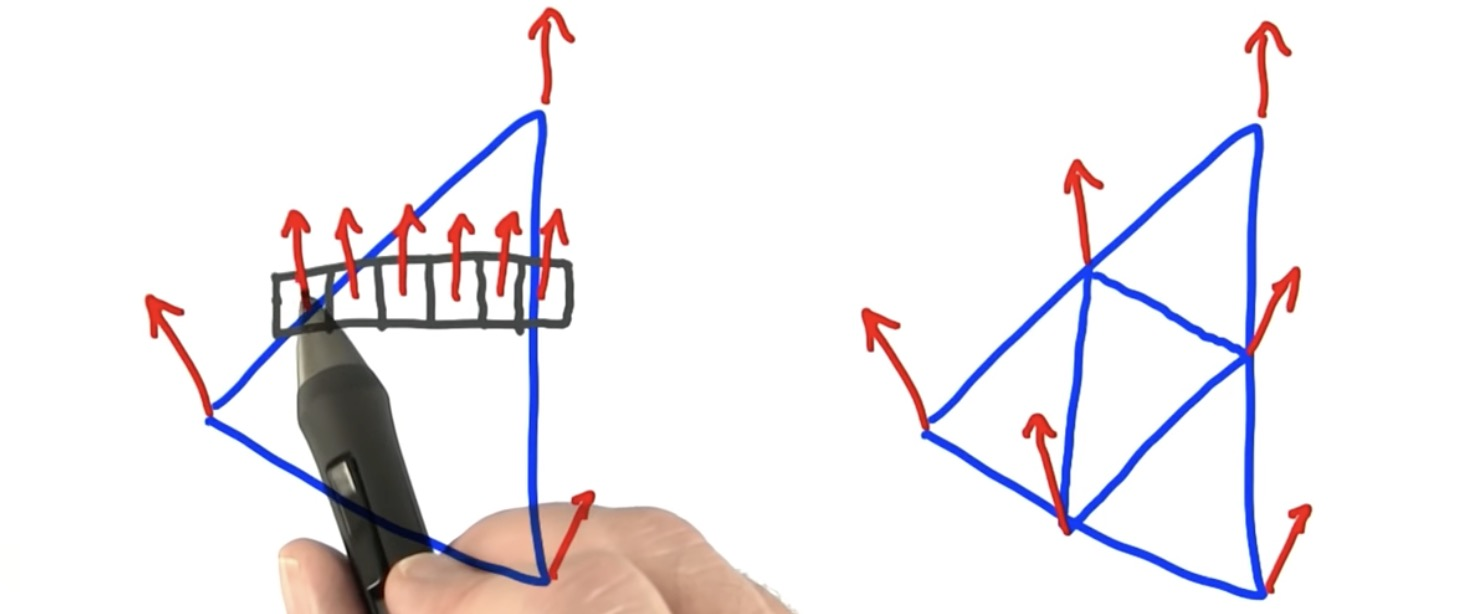
\includegraphics[width=0.7\textwidth]{imgs/phong_shade.png}
                \caption{Phong Shading}

            \end{figure}
            
        \end{itemize}
        
    \end{itemize}
    
    \item Recap of the graphics pipeline:
    \begin{itemize}
        \item Input: vertices in 3D space
        \item Vertex processing: MVP transforms, shading, texture mapping
        \item Triangle processing:
        \item Rasterization: Sampling triangle
        \item Fragment Processing: Z-buffer visibility tests, shading, texture mapping
        \item Framebuffer Operations:
    \end{itemize}
\end{itemize}

\section{Texture Mapping}

\begin{itemize}

    \item The texture pipeline:
    \begin{itemize}
        \item Three spaces: screen space, world space, texture space
        \item Projector function: project the surface's location into the texture coordinate space, usually $(u,v)$ space in the $[0,1]$ range.
        \item Corresponder function: converting texture coordinates to texture-space locations. \textbf{Wrapping mode} is usde to deal with the condition $(u,v)$ out of range $[0,1]$.
        
        Some common corresponder function: wrap, mirror, clamp (values outside the range $[0,1]$ are clamped to this range), border (texture coordinates outside $[0,1]$ are rendered with a separately defined border color).
    \end{itemize}
    
    
    \item Interpolation across triangles: barycentric coordinates
    
    From geometric viewpoint, $\alpha=\frac{A_A}{A_A+A_B+A_C},\beta=\frac{A_B}{A_A+A_B+A_C},\gamma=\frac{A_C}{A_A+A_B+A_C}$, where $A_i$ is the corresponding area.
    
    \begin{figure}[H]
        \centering
        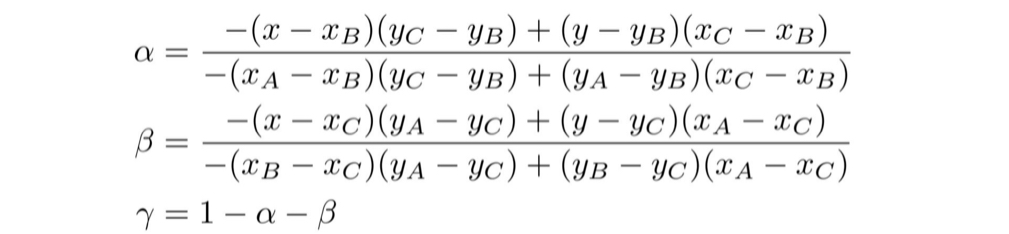
\includegraphics[width=0.7\textwidth]{imgs/barycentric_formula.jpeg}
    \end{figure}

    \begin{figure}[H]
        \centering
        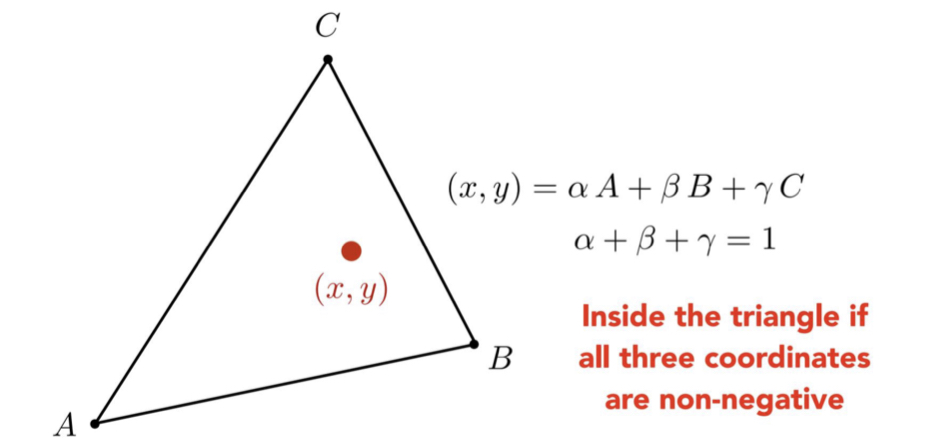
\includegraphics[width=0.7\textwidth]{imgs/barycentric.jpeg}
        \caption{Barycentric coordinates}
    \end{figure}
    
    \item Image Texturing: Each surface point is assigned a texture coordinate $(u,v)$.
    
    \item Magnification \& Minification:
\begin{itemize}
    \item  Magnification: Size of texel $>>$ Size of pixel. Num of texel $<<$ Num of pixel.
    \begin{itemize}
        \item Nearest neighbour (jaggy)
        \item bilinear interpolation (blured)
        \item take a smaller texel (good)
    \end{itemize}
    
    \item Minification: Size of texel $<<$ Size of pixel. Num of texel $>>$ Num of pixel.
    
    How to solve ? NN/Linear is not good. Lower the resolution of the texture.
    
    \item Mipmap: Image Pyramid, to solve magnification and minification.
    
    Mipmap may lead to \textbf{overblur} since mipmap is \textbf{square}.
    \begin{figure}[H]
        \centering
        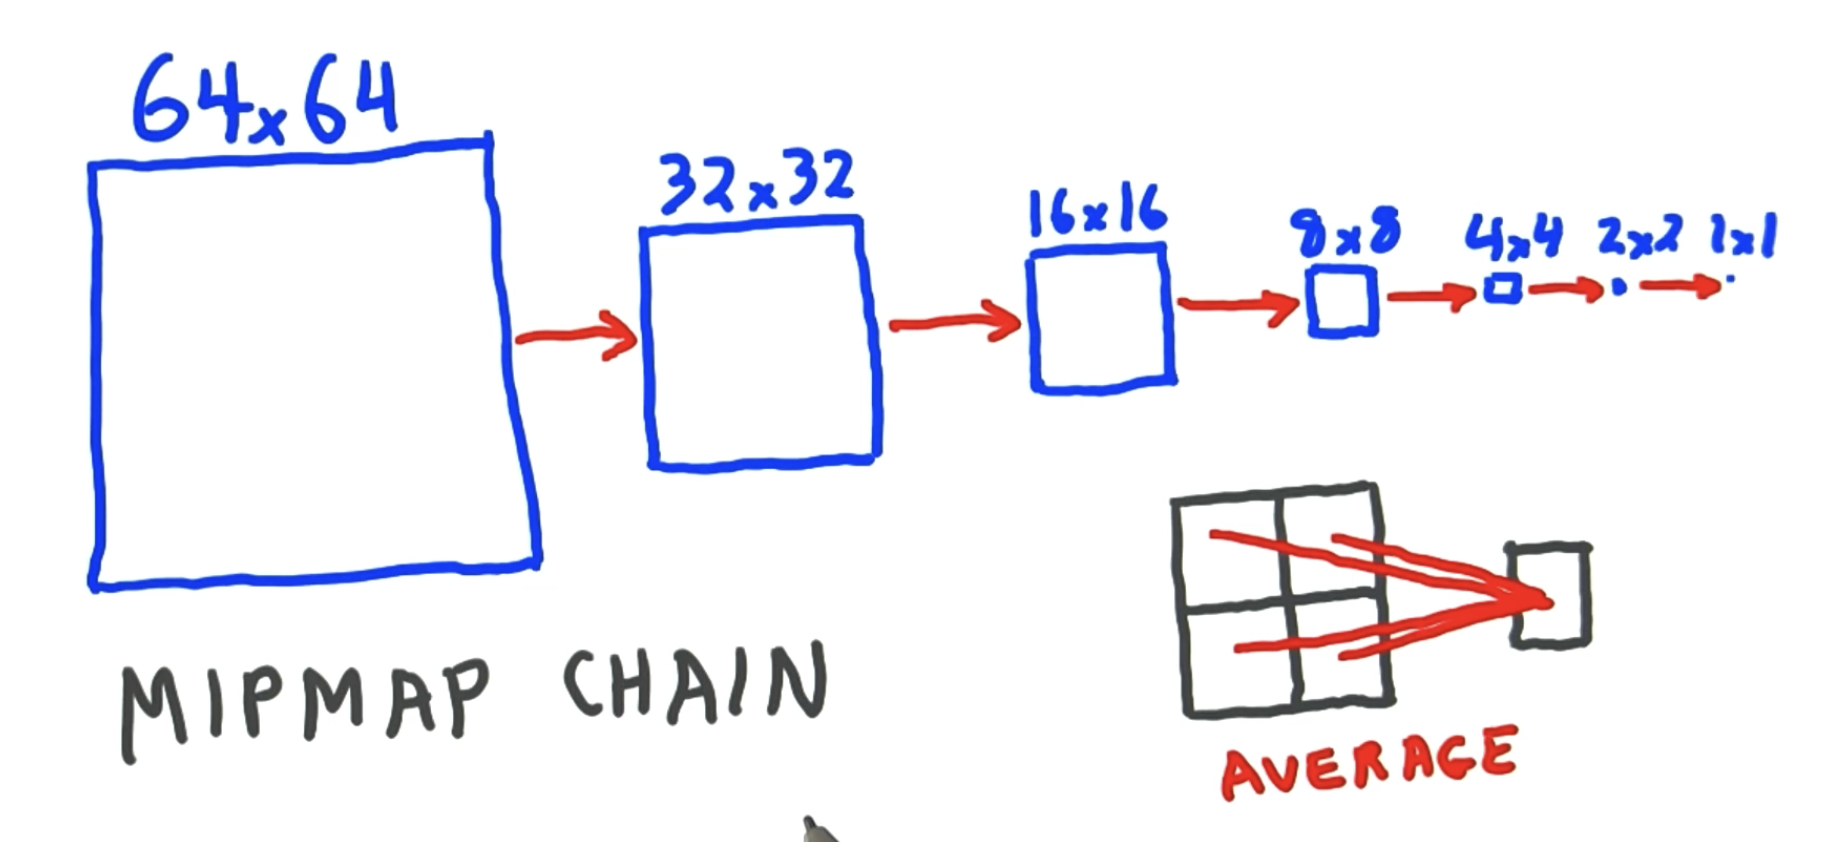
\includegraphics[width=0.7\textwidth]{imgs/mipmap.png}
    \end{figure}
    


\item Anisotropic Filtering: Better than Mipmap. Sample more on the direction with higher frequency.
\begin{figure}[H]
        \centering
        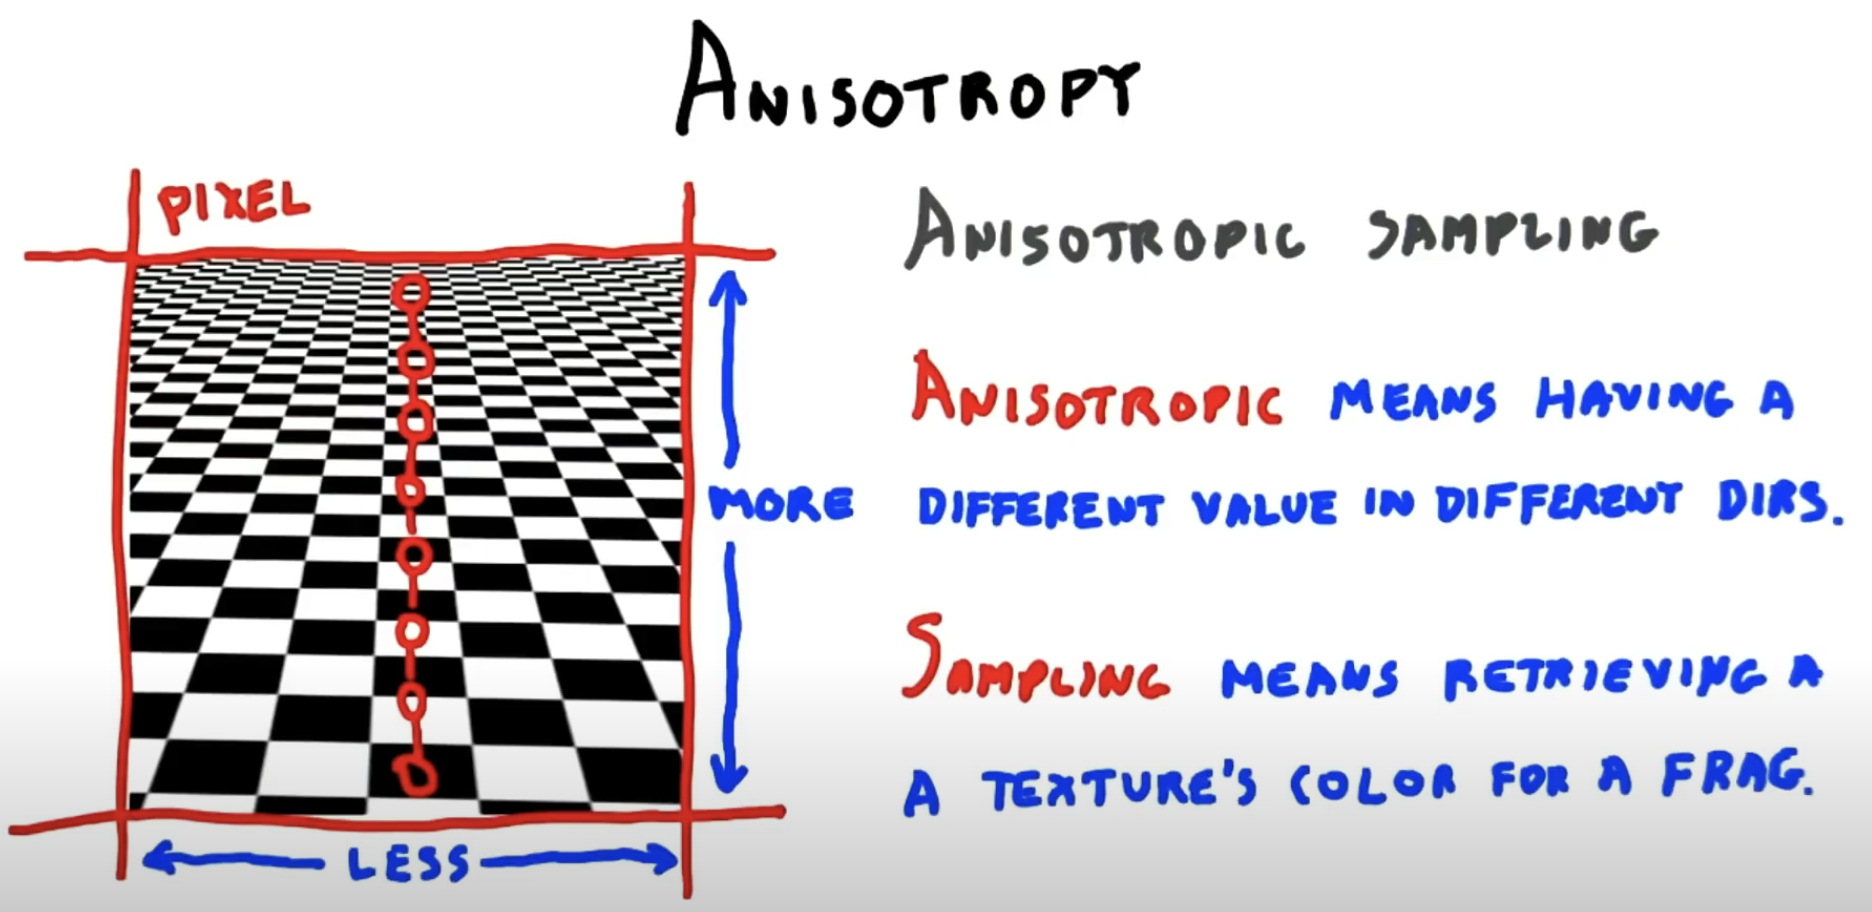
\includegraphics[width=0.7\textwidth]{imgs/ani_sample.png}
    \end{figure}
\item Unconstrained Anisotropic Filtering: Can be \textbf{not square}, compared to Mipmap.
 
  \end{itemize} 
  
 \item Bump Mapping:
 \begin{itemize}
     \item Three kinds of scales of features: Macro-features, Micro-features, Meso-features (mid-level).
     \item Bump mapping are used for Meso-features. \textbf{Adjust the shading parameters }at the pixel level.
     \item Key idea: \textbf{Modify the surface normal.}
     \item Details: a tangent frame, also called a tangent-space basis, is stored at each vertex. Store three vectors, vectex normal $n$, tanget $t$, bitangent $b$.
     
     \item One way is Blinn's methods: use a heightfield to modify the surface normal's direction
     \item Another way is Normal Mapping: directly store a normal map
 \end{itemize}
 
 \item Parallax Mapping:
 \begin{itemize}
     \item Why introduce Parallax Mapping? 
     
     A problem with bump and normal mapping is that the bumps never shift location with the view angle, nor ever block each other. (no occlusion)
     
     \item The key idea of parallax mapping is to take an educated guess of what should be seen in a pixel by examining the height of what was found to be visible.
     
     \item For parallax mapping, \textbf{the bumps are stored in a heightfield texture}.
 \end{itemize}
 
 \item Other applications: environment map, environment lighting...
 \item Exercises answers:
 
 \begin{figure}[H]
    \centering
    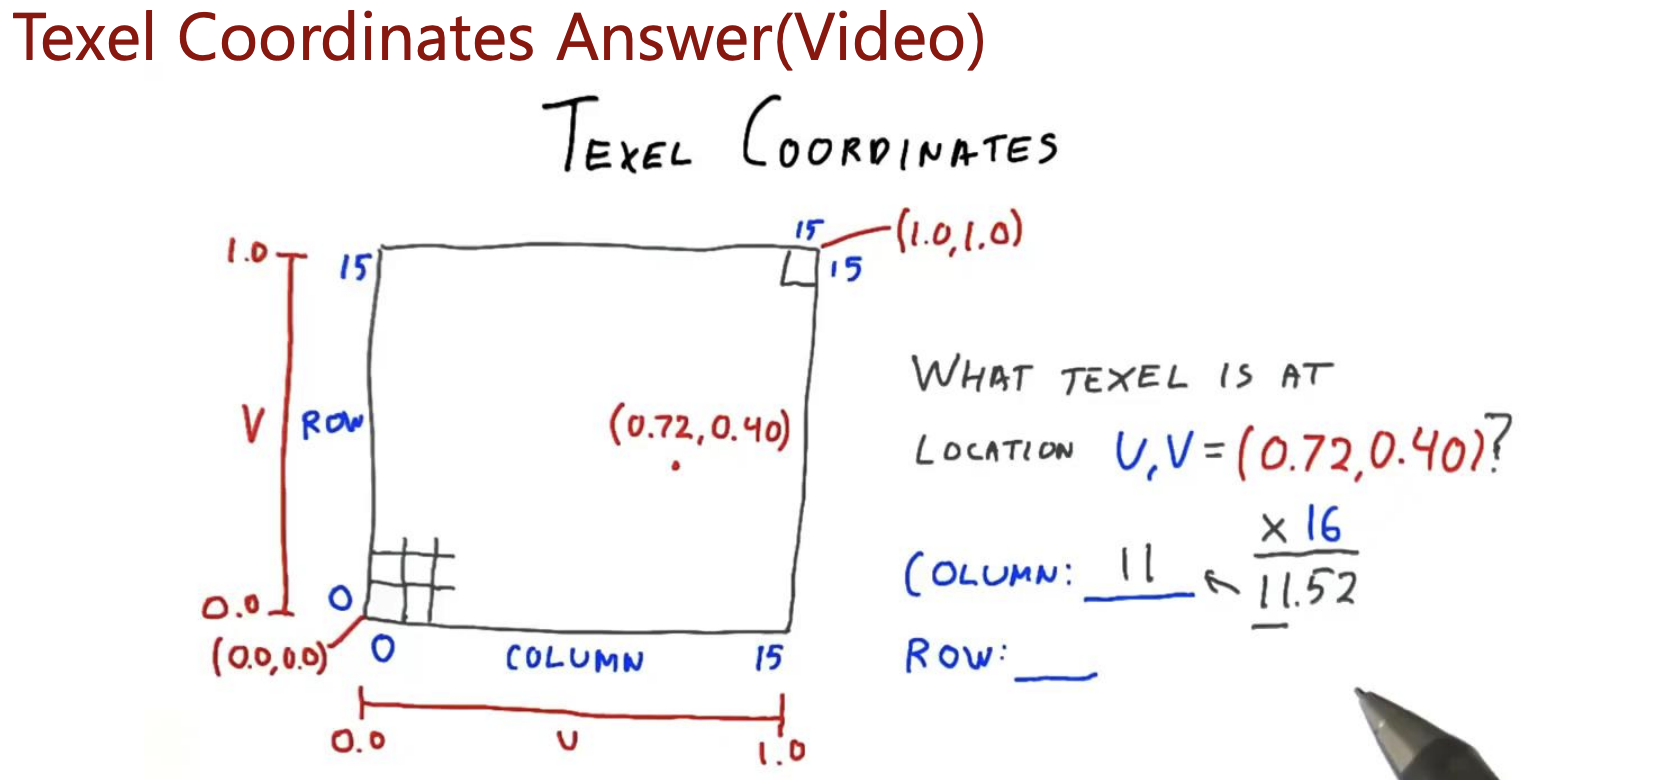
\includegraphics[width=0.7\textwidth]{imgs/ex1.png}
\end{figure}

 \begin{figure}[H]
    \centering
    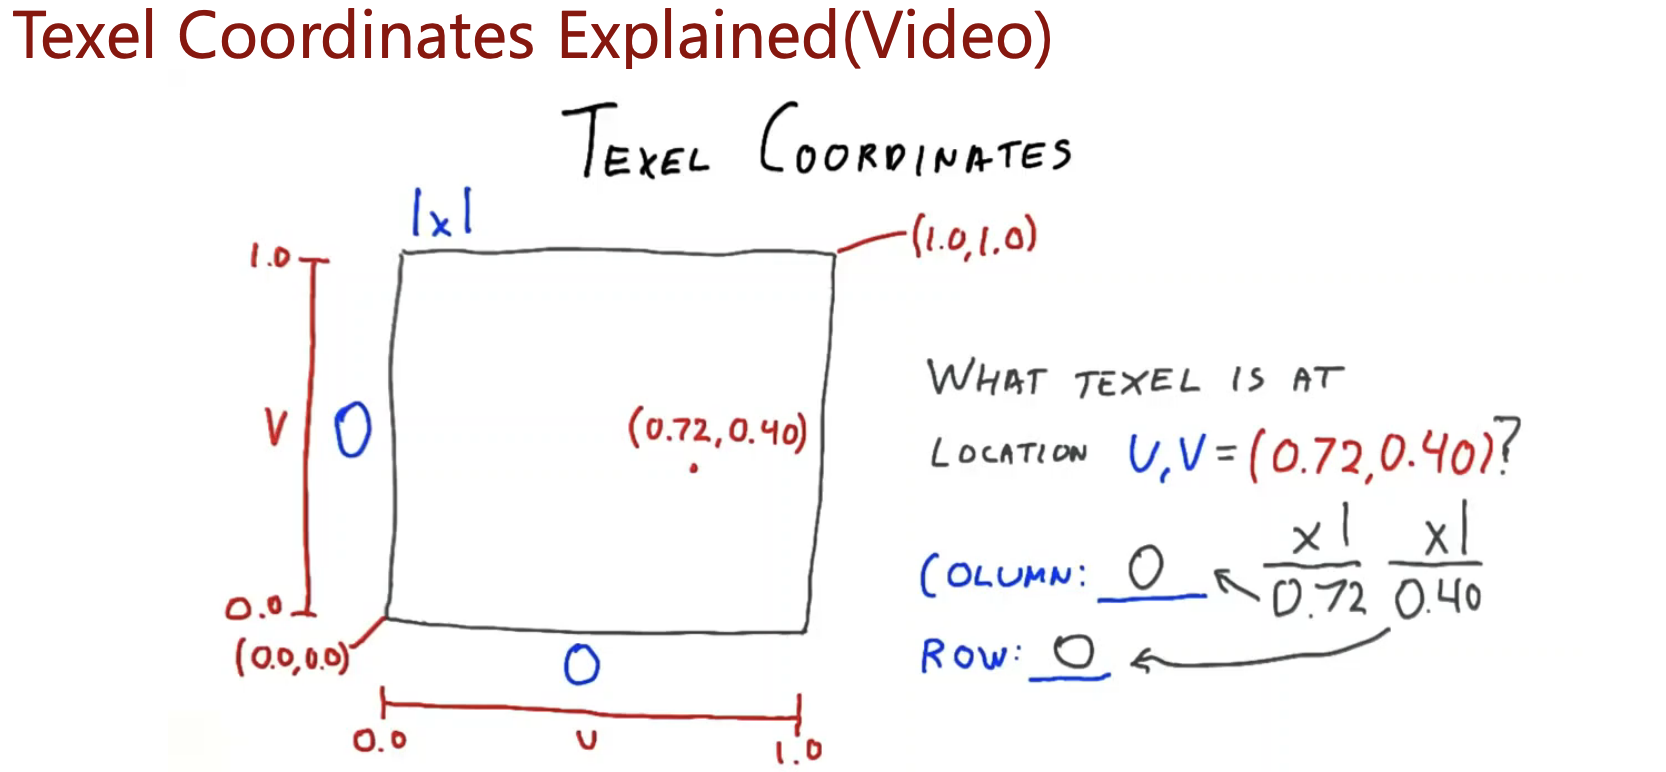
\includegraphics[width=0.7\textwidth]{imgs/ex2.png}
\end{figure}

 \begin{figure}[H]
    \centering
    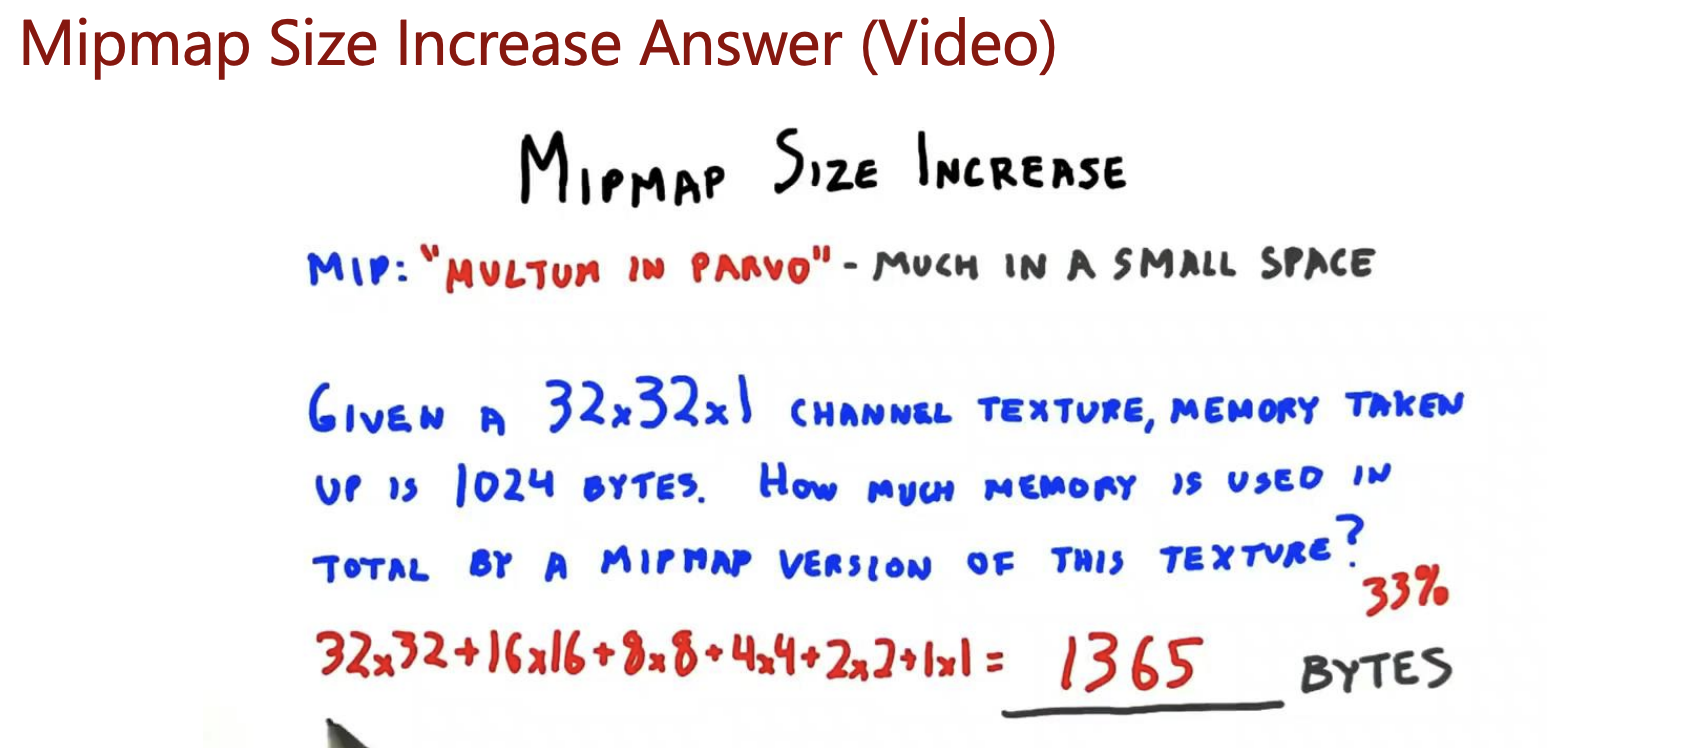
\includegraphics[width=0.7\textwidth]{imgs/ex3.png}
\end{figure}
 
\end{itemize}

\section{Geometry}

\subsection{Introduction to geometry}
\begin{itemize}
    \item Many ways to represent geometry:
    \begin{itemize}
        \item Implicit: sampling can be hard. Inside/outside tests can be easy.
        \item Explicit: sampling is easy. Inside/outside tests can be hard.
    \end{itemize}
    
    \item Implicit representations:
    \begin{itemize}
        \item Algebraic surface
        \item Constructive solid geometry: use $A$ and $B$, get $A\cup B$ and so on
        \item Distance function: TODO: understand this
        \item Level set methods: store a grid of values approximating function
        \item Fractals
    \end{itemize}
    
    \item Implicit representation pros and cons:
    \begin{itemize}
         \item Pros:  
         
         compact description (e.g., a function) 
         
         certain queries easy (inside object, distance to surface) 
         
         good for ray-to-surface intersection (more later) 
         
         for simple shapes, exact description / no sampling error 
         
         easy to handle changes in topology (e.g., fluid) 
         \item Cons: difficult to model complex shapes
    \end{itemize}
    
    \item Explicit representations:
    \begin{itemize}
        \item Point clouds
        
        \item Polygon mesh
        
        \item The wavefront object file format: a text file specifies vertices, normals, texture coordinates and their connectivities
    \end{itemize}
    
\end{itemize}

\subsection{Curves and Surfaces}
\begin{itemize}
    \item Bezier curves
    \item de Casteljau algorithm: repeat the interpolation to find the point
    \item Algebraic formula: Bernstein form. At each $t$, the summation of Bernstein polynomials is $1$.
    \begin{figure}[H]
        \centering
        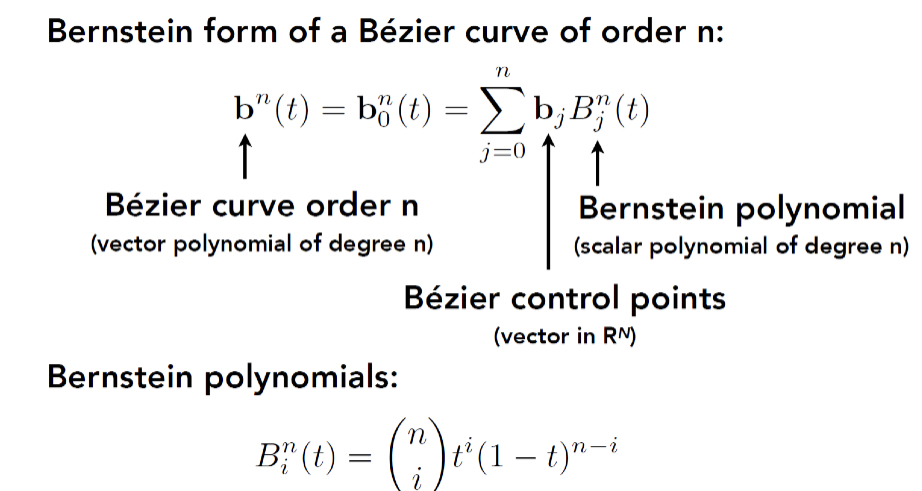
\includegraphics[width=0.7\textwidth]{imgs/bezier.jpeg}
    \end{figure}
    \item Properties:
    \begin{figure}[H]
        \centering
        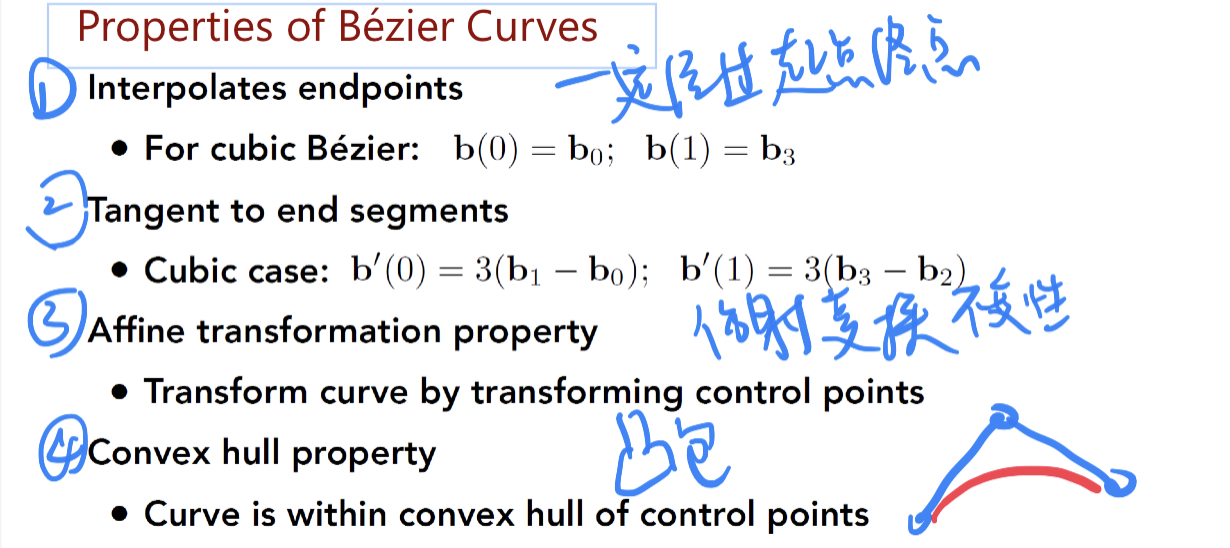
\includegraphics[width=0.7\textwidth]{imgs/bezier1.jpg}
    \end{figure}
    
    \item Piecewise Bezier curves: High order bezier curves are hard to control. Instead, we chain many low-order Bezier curve.
    
    $C_0$ continuity: $a_n=b_0$
    
    $C_1$ continuity: $a_n=b_0=\frac{1}{2}(a_{n-1}+b_1)$
    
    \item Bezier surface: TODO: understand this
    
\end{itemize}

\section{Geometry: Mesh}


\begin{itemize}
    \item Topology vs Geometry
    \begin{figure}[H]
        \centering
        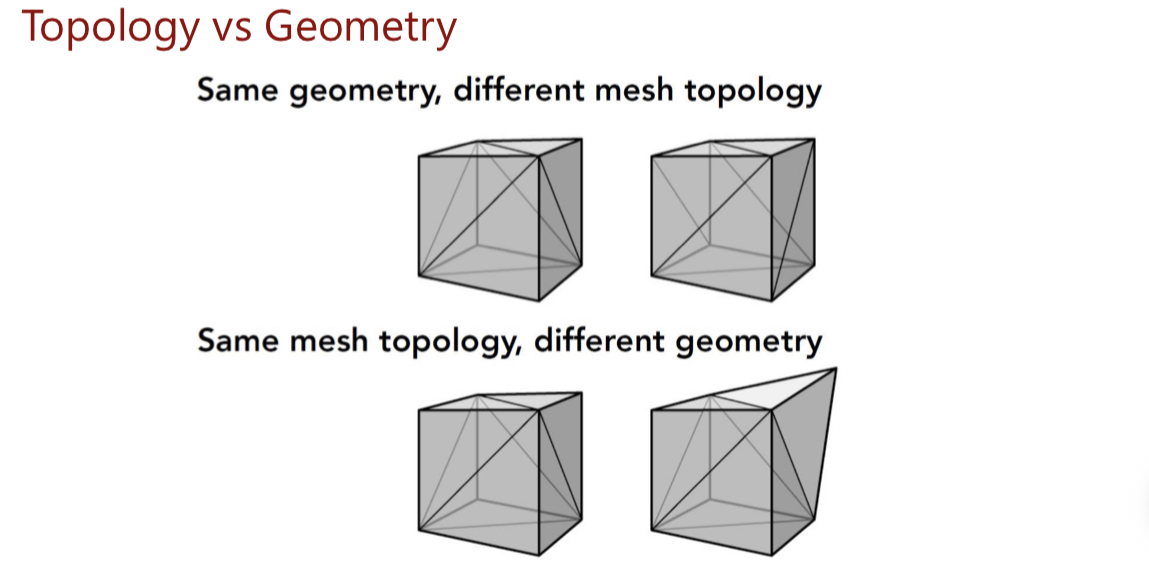
\includegraphics[width=0.7\textwidth]{imgs/mesh_vs_topo.jpeg}
    \end{figure}
    
    \item Local Mesh Operations: flip, split, collapse
    \item Global Mesh Operations: upsampling, downsampling,  sampling same number of triangles
    
    \item Loop Subdivision: 
    \begin{itemize}
        \item split each triangle into four
        \item Update for new vertices: $3/8*(A+B)+1/8*(C+D)$
        \begin{figure}[H]
        \centering
        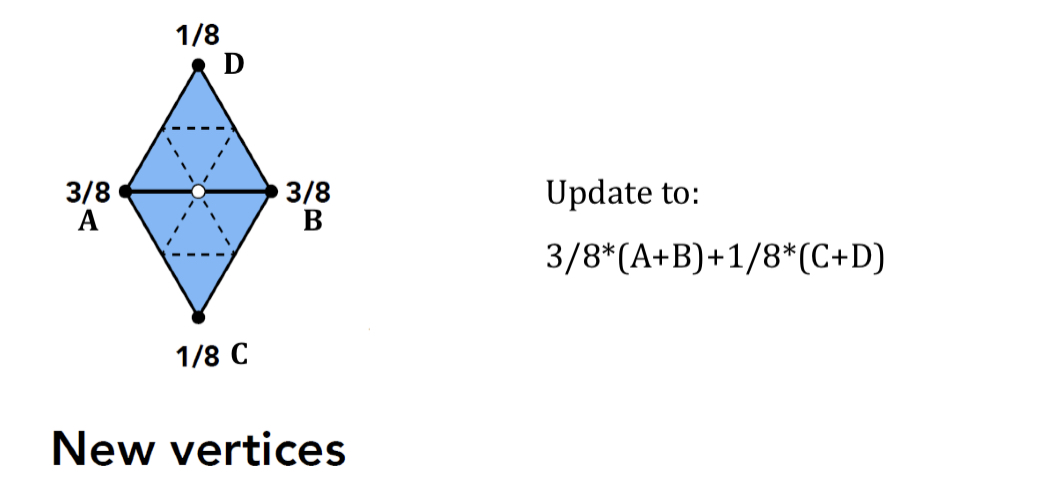
\includegraphics[width=0.7\textwidth]{imgs/update_new.jpeg}
    \end{figure}
        \item Update for old vertices: 
        \begin{figure}[H]
        \centering
        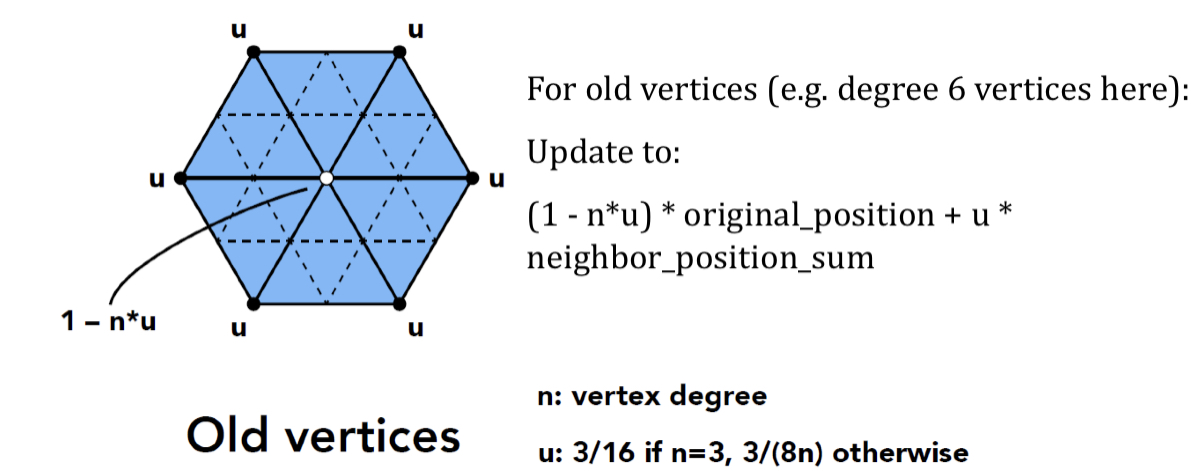
\includegraphics[width=0.7\textwidth]{imgs/update_old.jpeg}
    \end{figure}
    
    \end{itemize}
    
    \item Catmull-Clark Subdivision:
    \begin{itemize}
        \item Each subdivision step:
        
        Add vertex in each face
        
        Add midpoint on each edge
        
        Connect all new vertices
        
        \item Update rules:
        \begin{figure}[H]
        \centering
        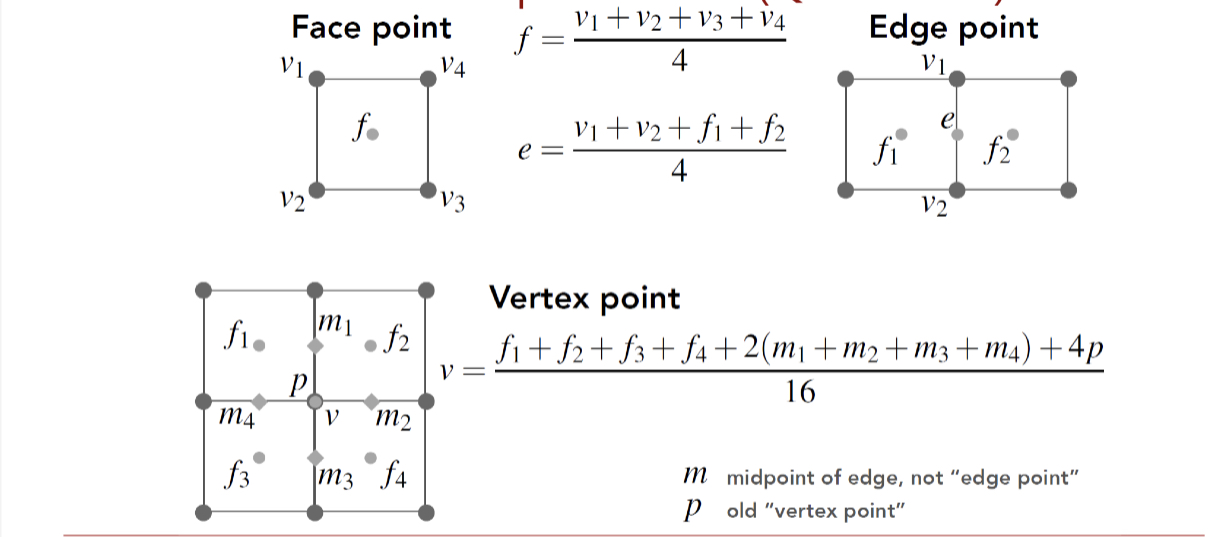
\includegraphics[width=0.7\textwidth]{imgs/cc_subdivide.jpeg}
    \end{figure}
    \end{itemize}
    
    \item Mesh Simplification: reduce number of mesh elements while maintaining overall shape
    
    \item Collapsing an edge:
    \begin{itemize}
        \item Quadric error metrics: new vertex should minimize its sum of square distance to previously related triangle planes
        
        \item Idea: compute edge midpoint, measure quadric error
        
        \item Better idea: choose point that minimizes quadric error
        \item Iteratively collapse edges 
        
        Which edges? Assign score with quadric error metric* 
        \begin{itemize}
            \item 
        
        approximate distance to surface as sum of distances to planes containing triangles 
        \item
        iteratively collapse edge with smallest score 
        \item
        greedy algorithm.. great results
        \end{itemize}
    \end{itemize}
    
    
\end{itemize}


\section{Ray Tracing}
\textbf{Note that this part is not well written.}
\begin{itemize}
    \item Ray Casting:
    
    1. Generate an image by casting one ray per pixel
    
    2. Check for shadows by sending a ray to the light
    
    \item Recursive (Whitted-Style) Ray Tracing:
    \begin{figure}
        \centering
        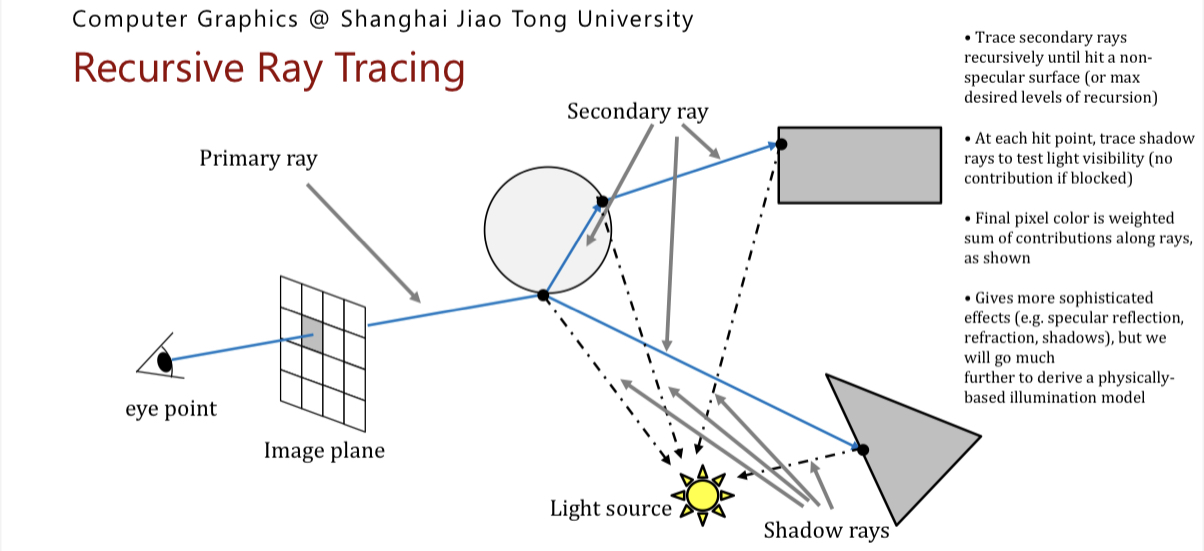
\includegraphics[width=0.7\textwidth]{imgs/ray_trace.jpeg}
    \end{figure}
    
    \item Ray-Surface Intersection
    \begin{itemize}
        \item Ray Equation:
        \item Ray intersection with sphere:
        \item Ray intersection with implicit surface:
        
        \item Ray intersection with triangle:
        
        \item Ray intersection with plane:
        
        \item Moller Trumbore algorithm:
    \end{itemize}
    
    \item Accelerating Ray-Surface Intersection:
    \begin{itemize}
        \item Bounding Volumes
        \item Uniform Spatial Partitions
        \item Spatial Partitions:
    \item Object Partitions:
    \end{itemize}
    
    
    
\end{itemize}



\end{document}
